%%%% Paramétrage du cours %%%%
\def\xxactivite{Cours}

\def\xxauteur{Emilien Durif -- Xavier Pessoles}
\fichefalse \proftrue \tdfalse \courstrue

\def\xxnumchapitre{Chapitre 7 \vspace{.2cm}}

\def\xxchapitre{Complexité algorithmique }

\def\xxcompetences{%
\textsl{%
\textbf{Savoirs et compétences :}\\
\begin{itemize}[label=\ding{112},font=\color{bleuxp}] 
\item Complexité.
\end{itemize}
}}

\def\xxfigures{
%
\includegraphics[width=\linewidth]{fractale}
%\\
%\textit{Modèle du pilote hydraulique avec pilotage interactif.}
}%figues de la page de garde

\input{\repRel/Style/pagegarde_cours_minitoc}
\setlength{\columnseprule}{.1pt}

\vspace{2cm}
\pagestyle{fancy}
\thispagestyle{plain}
\section{Préliminaire: parlons du temps\ldots{}}

\ldots{}ou plutôt des ordres de grandeur des durées.

On choisit comme unité la seconde\footnote{D'ailleurs, c'est l'unité de temps du système international} et on donne des logarithmes décimaux des durées étudiées.

Quelques repères à connaître.
\begin{enumerate}
\item  $\log_{10} t = x$ signifie $t = 10^{x}$, en particulier
$10^{n}\leq t < 10^{n+1}$ où $n = \floor{x}$.
\item $10^{0,5} = \sqrt{10} \approx 3$.
\item $10^{0,3} \approx 2$.
\item Un an vaut environ $3,15\times 10^{7}$s, \emph{i.e.} $\pi \,\mathrm{s} \approx 1$ nano-siècle.
\end{enumerate}

\begin{center}
  \begin{tabular}{rl rl}
   %\caption{Durées : ordre de grandeur (suite).}\\
  $\log_{10}(t)$ & Durée &   $\log_{10}(t)$ & Durée \\
  $-9,0$ & exécution d'une instruction &  $10,5$ & un millénaire\\
  $0,0$ & une seconde &  $13,1$ & âge de la maîtrise du feu\\
  $1,8$ & une minute &  $13,5$ & un million d'années\\
  $3,6$ & une heure &  $14,0$ & âge de Lucy\\
  $4,9$ & un jour &  $16,5$ & un milliard d'années\\
  $5,8$ & une semaine&  $17,0$ & âge de la vie sur Terre\\
  $6,4$ & un mois (30 jours)&  $17,6$ & âge de l'univers\\
  $7,5$ & un an &  $34,0$ & temps avant extinction des dernières étoiles\\
  $9,5$ & un siècle\\
\end{tabular}
\end{center}


\section{Introduction}

\begin{defi}{Complexité}
  La complexité algorithmique est l'étude des ressources requises pour exécuter un algorithme, en fonction d'un paramètre (souvent, la taille des données d'entrée). Les deux ressources en général étudiées sont :
\begin{itemize}
\item le temps nécessaire à l'exécution de l'algorithme;
\item la mémoire nécessaire à l'exécution de l'algorithme (en plus des données d'entrée).
\end{itemize}
\end{defi}

%\clearslide{}

%Nous avons déjà vu dans le TP06 que deux algorithmes résolvant un même problème peuvent avoir des temps d'exécution radicalement différents. 
%
%Nous allons étudier un exemple plus simple.

\subsection{Rappels d'arithmétique : le petit théorème de Fermat}

\begin{theorem}{Théorème de Fermat.}
  Soit $p$ un nombre premier et $a \in \ii{1,p}$, alors $a^{p-1} = 1 [p]$.
\end{theorem}

On s'intéresse au problème de l'étude de la primalité d'un entier naturel donné. 
Plusieurs méthodes existent pour répondre de manière déterministe à cette question, mais elles ne sont pas nécessairement satisfaisantes. 
Notamment, dire si un grand nombre entier est premier est assez difficile. 

On considérera alors le \og test \fg\ de primalité de Fermat, en base 2, en fonction d'un entier $p$.
\begin{itemize}
  \item On calcule $2^{p-1}$ modulo $p$. 
  \item Si cela ne donne pas $1$, $p$ n'est pas premier. 
  \item Si cela donne $1$, on dit que \og $p$ est probablement premier \fg.
\end{itemize}

\subsection{Algorithmes d'exponentiation}

La question qui se pose naturellement est de calculer $2^{p-1}$ modulo $p$ (sous entendu, sans exploiter l'exponentiation de Python). Voici trois manières différentes de le faire. 

\begin{enumerate}
  \item Une première idée est de calculer naïvement la puissance, de proche en proche, puis de considérer la division euclidienne de ce nombre par $p$.
\begin{lstlisting}
def expo1(p):
    """Renvoie 2**(p-1) mod p"""
    x = 1
    for i in range(p-1):
    	#Invariant : x=2**i
        x = 2*x
    return x % p
\end{lstlisting}
  \item Une seconde idée est de réaliser chaque multiplication modulo $p$, ce qui permet de ne multiplier que de \og petits \fg\ nombres à chaque fois. 
\begin{lstlisting}
def expo2(p):
    """Renvoie 2**(p-1) mod p"""
    x = 1
    for i in range(p-1):
    	#Invariant : x=2**i mod p
        x = (2*x) % p
    return x  
\end{lstlisting}
  \item Une troisième idée est de voir que si $n = 2k$, alors $2^n = \croch{\p{2^k}}^2$ et si $n = 2k+1$, alors $2^n = 2\croch{\p{2^k}}^2$. 
  Pour calculer une puissance (ici, de $2$), il suffit donc de calculer une puissance bien plus petite, suivie d'une mise au carré et d'une multiplication éventuelle. C'est l'idée de l'algorithme \emph{d'exponentiation rapide}.

\end{enumerate}
\begin{lstlisting}
def expo3(p):
    """Renvoie 2**(p-1) mod p par exponentiation rapide"""
    y = 1
    n = p-1
    x = 2
    while n > 0:
        # Invariant : y * (x**n) = 2**(p-1) mod p
        # Variant : n
        if n % 2 != 0: # n est impair
            y = (y * x) % p
            n = n - 1
        # n est pair et y * (x**n) = 2**(p-1) mod p
        x = (x * x) % p
        n = n // 2
    # n == 0 et y = 2 ** (p-1) modulo p
    return y
\end{lstlisting}


On a donc construit les \og tests \fg\ suivants.

\begin{lstlisting}
def premierprobable1(p):
    return expo1(p) == 1

def premierprobable2(p):
    return expo2(p) == 1

def premierprobable3(p):
    return expo3(p) == 1
\end{lstlisting}

\subsection{Temps d'exécution}

On se doute bien que :
\begin{enumerate}
\item les temps d'exécution varient en fonction du nombre $p$ à tester ;
\item il croissent avec $p$ (grosso-modo).
\end{enumerate}

%\clearslide{}
\'Etudions cela plus précisément, pour $i \in \ens{1,2,3}$ on note $T_i(p)$ le temps d'exécution de \texttt{premierprobablei(p)}.



Dressons un tableau des temps de calcul $T_{i}(n)$ pour les fonctions
que nous avions données, pour $i=1, 2, 3$.

%\clearslide{}
\begin{center}
\begin{tabular}{rrrr}
%\caption{Logarithmes des temps d'exécution (en secondes).\label{tab:tempsexpo}}\\
  %\toprule
 % $\log_{10}(p)$ & $\log_{10}(T_1(p))$& $\log_{10}(T_2(p))$ & $\log_{10}(T_3(p))$\\
%\midrule \endfirsthead
%\caption{Logarithmes des temps d'exécution (suite).}\\
%  \toprule
  $\log_{10}(p)$ & $\log_{10}(T_1(p))$& $\log_{10}(T_2(p))$ & $\log_{10}(T_3(p))$\\
%\midrule \endhead
% $1$     & $-5,4$        & $-5,3$        & $-5,2$\\
% $2$     & $-4,7$        & $-4,6$        & $-5,1$\\
% $3$     & $-3,7$        & $-3,6$        & $-4,9$\\
%$4$     & $-2,5$        & $-3,0$        & $-4,8$\\
%$5$     & $-0,7$        & $-2,0$        & $-4,8$\\
$6$     & $1,2$         & $-1,0$        & $-4,7$\\
%$7$     &$\mathit{3,2}$   & $0,0$         & $-4,6$\\
$8$     &$\mathit{5,2}$   & $1,0$         & $-4,6$\\
$9$     &$\mathit{7,2}$   & $\mathit{2,0}$  & $-4,5$\\
$10$    & $\mathit{9,2}$  & $\mathit{3,0}$  & $-4,4$\\
%$11$    & $\mathit{11,2}$ & $\mathit{4,0}$  & $-4,3$\\
$14$    & $\mathit{17,2}$ & $\mathit{7,0}$  & $-4,3$\\
$24$    & %$\mathit{37,2}$
                        & $\mathit{17,0}$ & $-4,0$\\
$100$ & & %$\mathit{93}$
                        & $-2,9$\\
$2000$ & & & $0,0$\\
%\bottomrule
\multicolumn{4}{c}{\emph{(les valeurs en italique sont des extrapolations)}}\\
\end{tabular}
\end{center}

Ces temps varient \textbf{énormément} en fonction de l'algorithme utilisé.
%\clearslide{}
Suivant l'algorithme, on a une exécution quasi-instantanée ou au contraire interminable.

Ainsi, avoir une idée du temps d'exécution d'un programme est nécessaire avant
de l'utiliser réellement dans un contexte scientifique ou industriel.

Ainsi, étudier expérimentalement le temps de calcul d'un algorithme est :
\begin{enumerate}
\item nécessaire pour «valider» l'usage d'un algorithme;
\item insuffisant pour trouver\footnote{En inventant un
    algorithme ou en combinant des algorithmes existants} des algorithmes performants.
\end{enumerate}

%\clearslide{}
\begin{center}
\textbf{Il est donc nécessaire d'étudier théoriquement la complexité
  des algorithmes.}  
\end{center}

%\clearslide{}
Comment faire cette étude théorique?

\begin{enumerate}
\item On se donne un \emph{modèle} de l'exécution des programmes. Ce modèle précise le temps de calcul de chaque opération élémentaire.
\item Il ne reste plus qu'à regarder, pour un programme donné, combien d'instructions élémentaires il effectue.
\end{enumerate}

%\clearslide{}
\section{Étude théorique}


\subsection{Deux mauvaises nouvelles}

\begin{enumerate}
\item Compter exactement le nombre d'opérations faites par le programme est pénible voire difficile (mathématiquement).
\item Savoir précisément combien de temps met chaque opération élémentaire est difficile et change suivant les machines.
\end{enumerate}

\subsection{Deux bonnes nouvelles}

\begin{enumerate}
\item Il n'est pas nécessaire d'être extrêmement précis : on se  contente d'un ordre de grandeur quand le paramètre devient grand. On
  parle d'\textbf{estimation asymptotique de la complexité}.
\item Les principes de cette estimation étaient déjà
  valables il y a $70$ ans\footnote{Le Harvard Mark III, construit en
    1949, était  l'ordinateur le plus rapide du
    monde. Il avait coûté de l'ordre de $10^{5}$\$ à l'époque, soit
    $10^{6}$\$ actuels. Il faisait une addition en $4\times 10^{-3}$s
    et avait environ $8$ko de mémoire vive. Depuis les performances
    des ordinateurs ont été multipliées par $10^{6}$ environ.} et le
  seront encore probablement dans $50$ ans.
\end{enumerate}

%\clearslide{}
\subsection{Étude théorique de \texttt{premierprobable2}}

\begin{lstlisting}
def expo2(p):
    """Renvoie 2**(p-1) mod p"""
    x = 1
    for i in range(p-1):
        x = (2*x) % p
    return x  
    
def premierprobable2(p):
    return expo2(p) == 1
\end{lstlisting}

Comment estimer le temps d'exécution de \texttt{premierprobable2(p)}?

%\clearslide{}
Les opérations effectuées dans \texttt{premierprobable2(p)} sont les suivantes.
\begin{itemize}
\item[\textbullet] Une affectation.
\item[\textbullet] Une boucle effectuant $\texttt{p}-1$ tours. À chaque tour on
  effectue les opérations suivantes :
  \begin{itemize}
  \item une multiplication ;
  \item un calcul de reste ;
  \item une affectation.
  \end{itemize}
\item[\textbullet] Une comparaison.
\end{itemize}

%\clearslide{}
On considère le modèle usuel suivant.

\begin{itemize}
\item[\textbullet] Le temps mis par une affectation est constante.
\item[\textbullet] Le temps mis par opération arithmétique (somme, produit,
  division, calcul de reste) est constant.
\item[\textbullet] Le temps mis par une comparaison de deux nombres est constant.
\end{itemize}

%\clearslide{}
Appelons alors
\begin{itemize}
\item[\textbullet] $c_{1}$ le temps d'une affectation;
\item[\textbullet] $c_{2}$ le temps d'une multiplication;
\item[\textbullet] $c_{3}$ le temps d'un calcul de reste;
\item[\textbullet] $c_{4}$ le temps d'une comparaison.
\end{itemize}

Cela donne,
$ \quad   T_{2}(p) = c_{1} + (p-1) (c_{2} + c_{3} + c_{1}) + c_{4}$.

%\clearslide{}

C'est une expression déjà un peu compliquée et qui, à première vue,  ne nous apprend pas grand-chose, car on ne  connaît pas les constantes en jeu.
Ces constantes dépendent de la machine sur lequel on  exécutera le programme. 

On a quand même une information intéressante : $T_{2}(p)$ n'augmente pas plus vite que $p$ multipliée par une constante.

%Montrons ce second point. Pour $p\geq 1$ : 
%
%$ \left |\begin{array}{ll}
%\text{On a vu que } & T_{2}(p) = c_{1} + (p-1) (c_{2} + c_{3} + c_{1}) + c_{4}. \\
%\text{De plus} & pc_{1}> c_{1}, p (c_{2} + c_{3} + c_{1}) > (p-1) (c_{2} + c_{3} + c_{1}) \text{ et  } pc_{4}>c_4. \\
%\text{Au final }&    T_{2}(p) \leq c_{1}p + p(c_{2}+c_{3}+c_{1})+c_{4}p\\
%\text{et }  & T_{2}(p)\leq (2c_{1}+c_{2}+c_{3}+c_{4})p.
%  \end{array}\right.$
%  
  
Montrons ce second point. Pour $p_0\geq 1$ : 
$ \left |\begin{array}{ll}
\text{On a vu que } & T_{2}(p) = c_{1} + (p-1) (c_{2} + c_{3} + c_{1}) + c_{4}. \\
\text{De plus} & p_0c_{1}> c_{1}, p_0 (c_{2} + c_{3} + c_{1}) > (p-1) (c_{2} + c_{3} + c_{1}) \text{ et  } p_0c_{4}>c_4. \\
\text{Au final }&    T_{2}(p) \leq c_{1}p_0 + p_0(c_{2}+c_{3}+c_{1})+c_{4}p_0\\
\text{et }  & T_{2}(p)\leq (2c_{1}+c_{2}+c_{3}+c_{4})p_0.
  \end{array}\right.$
  

%\clearslide{}

On a donc montré qu'il existait un entier $p_{0}$ et un réel $C>0$ tel que
$  \forall p\geq p_0 \qquad T_{2}(p)\leq Cp_0$.

On dit alors que $T_{2}(p)$ est \emph{dominé} par $p$ et on note
$  T_{2}(p) = O(p)$.

%\clearslide{}
\begin{defi}{}
  On dit qu'une suite $(u_{n})$ est dominée par une suite $(v_{n})$ et
  on note $u_{n} = O(v_{n})$ si,  à partir d'un certain rang, la suite
  $(u_{n}/v_{n})$ est bien définie et bornée.  
\end{defi}

Ici, on a, pour $p\geq 1$: $0 \leq T_{2}(p) \leq C p$; donc $ \abs{\frac{T_{2}(p)}{p}} \leq C$ et $T_{2}(p)=O(p)$.

\begin{rem}
  Bien entendu, on a aussi $T_2(p) = O(p^2)$, même si cela ne nous intéresse pas ... Nous aimerions donc bien aussi certifier qu'il existe une constante $C'$ telle que, pour tout $p\geq 1$, $C'p \leq T_2(p)$. 
  Cela se traduirait par $p = O(T_2(p))$. Conjugué avec $T_2(p) = O(p)$, cela se note $T_2(p) =\Theta(p)$. 
  
  Souvent, obtenir une telle borne inférieure est bien plus difficile qu'obtenir une majoration, nous ne nous en soucierons généralement pas. 
\end{rem}


%\clearslide{}
\subsection{Rédaction}
Nous avons détaillé l'étude de \texttt{premierprobable2}. On peut aller
beaucoup plus vite.

Il suffit de dire:

\begin{enumerate}
\item On considère que les temps d'exécution d'une affectation, d'une
  opération arithmétique et d'une comparaison sont constant.
\item Dans \texttt{premierprobable2(p)}, on effectue une affectation et
  une comparaison ainsi que $(\texttt{p}-1)$ tours de boucle, avec un
  nombre constant d'opérations de temps constant à chaque tour.
\item Donc le temps d'exécution de \texttt{premierprobable2(p)} est un
  $O(\texttt{p})$.
\end{enumerate}

%\clearslide{}
\subsection{Étude expérimentale de \texttt{premierprobable2}}
Pour $p = \floor{\dfrac{p_0}{q^k}}$, avec $q = 1,35$, $p_0 = 10^7$ et $k\in\ii{0,20}$, on calcule $T_2(p)$ et l'on effectue ensuite une régression linéaire par moindres carrés.

\begin{minipage}[c]{.48\linewidth}
Cette étude expérimentale (voir figure ci-contre)%~\ref{fig.pp2})  
  nous donne :$ T_{2}(p)\approx b_{2} p^{\alpha_{2}}$ où $\alpha_{2}\approx 1,005$ 
   et $b_{2} = 10^{\beta_{2}}$ $\approx 10^{-7,16}$ $\approx 6,9\times 10^{-8}$.

\begin{itemize}
\item[\textbullet] La constante $b_{2}$ ne pouvait de toute façon pas être prédite
  par notre étude théorique.
\item[\textbullet] On est (à peu de choses près) sur du $O(p)$. La différence vient
  d'erreurs liées à notre modèle et aux erreurs expérimentales.
\item[\textbullet] Si on prend comme référence qu'une instruction machine prend
  un temps $t = 10^{-9}s$, l'étude expérimentale semble montrer que
  $T_{2}(p)\approx 70 p \times t$.
\end{itemize}
\end{minipage}\hfill
\begin{minipage}[c]{.48\linewidth}
%\begin{figure}%[!h]
  \begin{center}
%\centering
    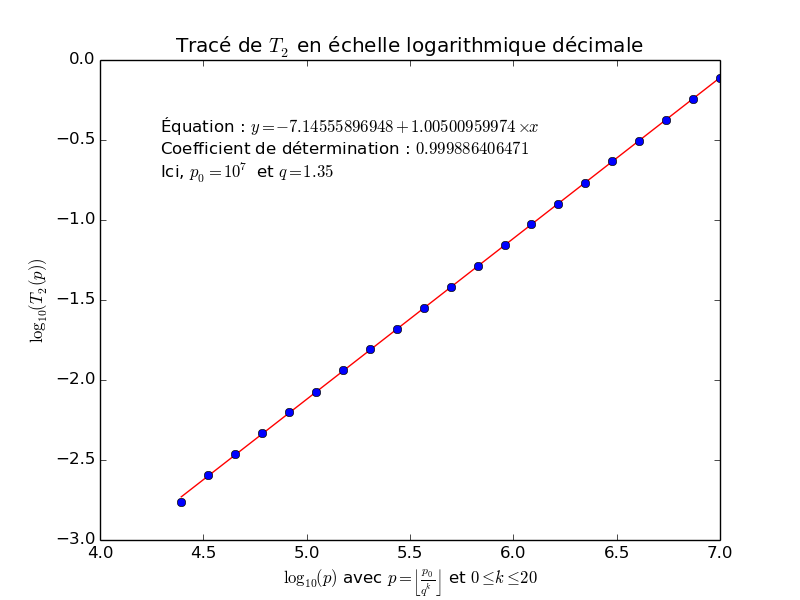
\includegraphics[width=\linewidth]{pp2.png}
    %\caption{Tracé expérimental de $T_2$ en échelle logarithmique décimale.}
%    \label{fig.pp2}
 \end{center}
%\end{figure}
\end{minipage}

\begin{rem}
  Ce n'est pas toujours la quantité $p$ qui est pertinente, mais plutôt la taille qu'occupe l'entier $p$ en mémoire, qui est de l'ordre de $\log_2(p)$.
\end{rem}

%\clearslide{}

\subsection{Étude théorique de \texttt{premierprobable3}}

\begin{lstlisting}
def expo3(p):     
    """Renvoie 2**(p-1) mod p par exponentiation rapide"""
    y = 1
    n = p-1
    x = 2
    while n > 0:
        # Invariant : y * (x**n) = 2**(p-1) mod p
        # Variant : n
        if n % 2 != 0: # n est impair
            y = (y * x) % p
            n = n - 1
        # n est pair et y * (x**n) = 2**(p-1) mod p
        x = (x * x) % p
        n = n // 2
    # n == 0 et y = 2 ** (p-1) modulo p
    return y
def premierprobable3(p):
    return expo3(p) == 1
\end{lstlisting}


On effectue un nombre constant d'opérations de temps constant, puis
une boucle \texttt{while} effectuant à chaque tour un nombre borné
d'opérations de temps constant, puis une comparaison.

Toute la difficulté est d'estimer le nombre de tours effectués par la
boucle.
\begin{itemize}
\item[\textbullet] Il est inférieur ou égal à $p$ ($n$ est un variant de la
  boucle et est initialisé à $p-1$), donc $T_{3}(p)=O(p)$.
\item[\textbullet] En fait $n$
  est divisé (au moins) par deux à chaque tour de boucle. Donc
  $\floor{\log_{2}(n)}$ est un variant de boucle.
\item[\textbullet] Donc on effectue au
  plus $1+ \floor{\log_{2}(p-1)}$ $= O(\log_{2}(p)) =$ $ O(\log p)$ tours de boucle.
\end{itemize}
Donc $T_{3}(p) = O(\log p)$.


%\clearslide{}
\subsection{Comparaison avec l'étude expérimentale}

\begin{minipage}[c]{.48\linewidth}
Pour $p = \floor{\dfrac{p_0}{q^k}}$, avec $q = 140$, $p_0 = 10^{140}$ (!!) et $k\in\ii{0,20}$, on calcule $T_3(p)$ et l'on effectue ensuite une régression linéaire par moindres carrés. Cette étude expérimentale 
(voir figure ci-contre) 
%(voir figure~\ref{fig.pp3}) 
nous donne :
$T_{3}(p)$ et $\log p$ une relation affine :
$  T_{3}(p) \approx \alpha_{3}\log_{10} p + \beta_{3}$. Donc $T_{3}(p)$ semble bien être un $O(\log p)$.

NB: en général, quand on note $\log$, il faut comprendre
\begin{itemize}
\item $\ln$ si c'est dans un texte de mathématiques en anglais;
\item $\log_{10}$ si c'est dans un texte de mathématiques ou de
  physique en français ;
\item $\log_{2}$ si c'est dans un texte d'informatique.
\end{itemize}

\end{minipage} \hfill
\begin{minipage}[c]{.48\linewidth}
%\begin{figure}[!h]
  \begin{center}
    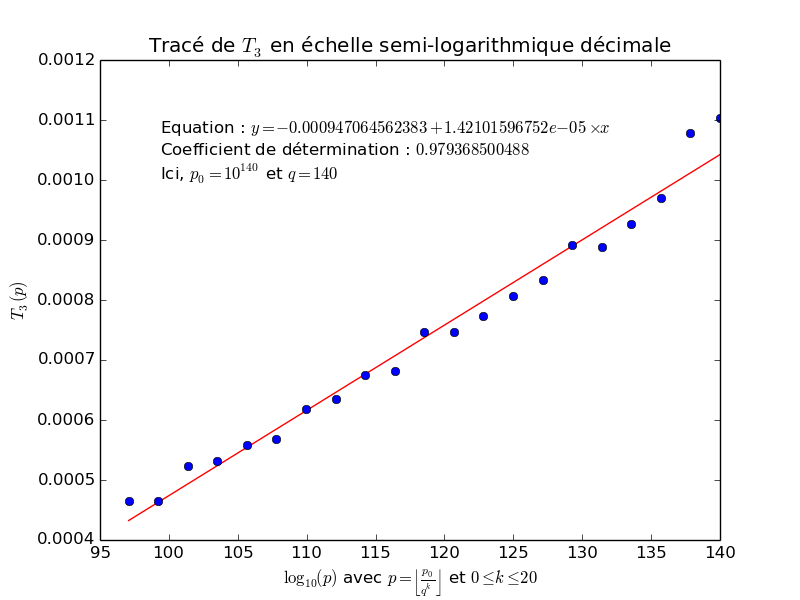
\includegraphics[width=\textwidth]{pp3.png}
    %\caption{Tracé expérimental de $T_3$ en échelle semi-logarithmique décimale.}
   % \label{fig.pp3}
  \end{center}
%\end{figure}
\end{minipage}

Mais de toute façon, ici on cela n'a pas d'importance car pour tout $x>0$, $ \ln x = \ln 2 \, \log_{2} x = \ln 10\, \log_{10}x$.

Donc $ O(\ln n) = O(\log_{2} n) = O(\log_{10} n)$.

\subsection{Étude théorique de \texttt{premierprobable1}}


\begin{lstlisting}
def expo1(p):
    """Renvoie 2**(p-1) mod p"""
    y = 1
    for i in range(p-1):
        y = 2*y
    return y % p

def premierprobable1(p):
    return expo1(p) == 1
\end{lstlisting}

%\clearslide{}
\begin{itemize}
\item[\textbullet] On considère que les temps d'exécution d'une affectation, d'une
  opération arithmétique et d'une comparaison sont constants.
\item[\textbullet] Dans \texttt{premierprobable1(p)}, on effectue une affectation, un
  calcul de reste et
  une comparaison ainsi que $(\texttt{p}-1)$ tours de boucle, avec un
  nombre constant d'opérations de temps constant à chaque tour.
\item[\textbullet] Donc le temps d'exécution de \texttt{premierprobable1(p)} est un
  $O(\texttt{p})$.
\end{itemize}

%\clearslide{}
\subsection{Étude expérimentale de \texttt{premierprobable1}}

\begin{minipage}[c]{.48\linewidth}
Pour $p = \floor{\dfrac{p_0}{q^k}}$, avec $q = 1,35$, $p_0 = 3\times 10^5$ et $k\in\ii{0,20}$, on calcule $T_1(p)$ et l'on effectue ensuite une régression linéaire par moindres carrés. Cette étude expérimentale 
(voir figure ci-contre)
%(voir figure~\ref{fig.pp2}) 
nous donne :
$  T_{1}(p)\approx b_{1} p^{\alpha_{1}}$ où $\alpha_{1}\approx 1,76$
et  $b_{1} = 10^{\beta_{1}} \approx 10^{-9,52}  \approx 3,02 \times 10^{-10}$.

Il semble alors que $T_1(p)$ n'est pas en $O(p)$ !!!

Les causes possibles:
\begin{itemize}
\item[\textbullet] cela peut provenir d'erreurs expérimentales. Mais ici, l'erreur paraît vraiment 
élevée;
\item[\textbullet] le modèle peut être erroné : les opérations sont-elles vraiment de temps constant~?
\end{itemize}
\end{minipage} \hfill
\begin{minipage}[c]{.48\linewidth}
%\begin{figure}[!h]
  \begin{center}
    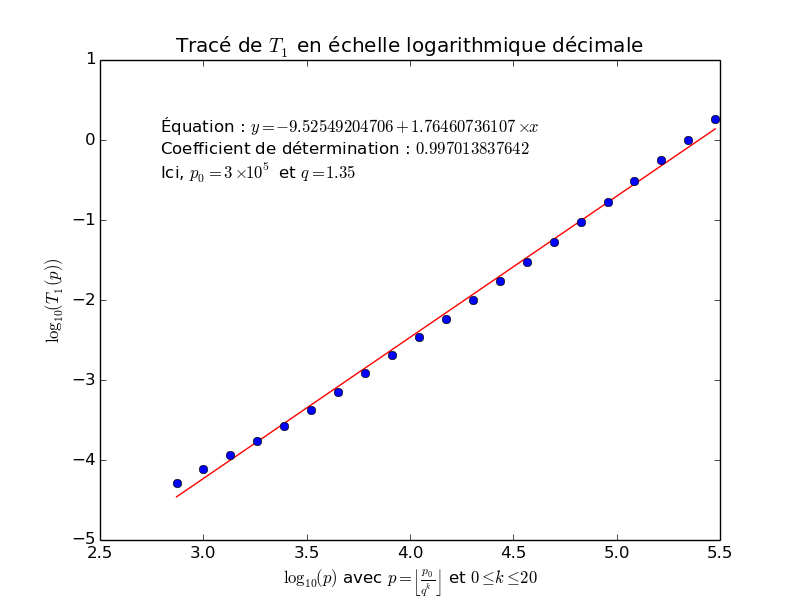
\includegraphics[width=\textwidth]{pp1.png}
    %\caption{Tracé expérimental de $T_1$ en échelle logarithmique décimale.}
%    \label{fig.pp1}
  \end{center}
\end{minipage} 




Ici, les nombres manipulés sont très grands puisqu'on calcule
$2^{p-1}$. Or, $2^{p-1}$ possède environ $\log_{10} (2^{p-1}) =
(p-1)\log_{10} 2$ chiffres.

Une hypothèse : chaque multiplication de \texttt{y} par $2$ coûte un temps proportionnel à la longueur de \texttt{y}, est en temps $C \log \texttt{y}$.

%\clearslide{}
Au $i\ieme$ tour de boucle, \texttt{y} vaut $2^{i}$, donc le temps de
calcul de la multiplication est $C i \log 2$. Donc le temps de calcul
de l'ensemble de la boucle est $\quad   \sum_{i=0}^{p-2} C i \log 2 \leq (p-1) C (p-2)\log 2\leq p^{2}C\log 2$.
Donc le temps de calcul de l'ensemble de la boucle est un $O(p^{2})$.

%\clearslide{}
Il reste à estimer le temps de calcul du reste de $2^{p-1}$ dans la
division par $p$. On peut penser que ce temps de calcul est au plus
proportionnel au nombre de chiffres de $2^{p-1}$ multiplié par le
nombre de chiffres de $p$, donc est dominé par $p\log p$, donc par
$p^{2}$.

Au final, le temps de calcul serait donc un $O(p^{2})$.

%\clearslide{}
Retour sur l'expérimentation:
\begin{itemize}
\item[\textbullet] On trouve un $O(p^{1,76})$, ce qui est déjà plus proche de $O(p^{2})$.
\item[\textbullet] Si on regarde la courbe expérimentale, on a l'impression qu'elle
  est plutôt convexe. Comme ce qui nous intéresse est la pente pour
  $p$ élevé, on peut penser que nous l'avons expérimentalement sous-estimée.
\end{itemize}
%\clearslide{}

\section{\'Etude dans le pire des cas}

Revenons sur la recherche d'un élément dans un tableau (fait dans le cours sur les tableaux). 

\begin{lstlisting}
def appartient(e, t):
    """Retourne un booléen disant si e appartient à t
       Précondition : t est un tableau"""
    for x in t:
        # Invariant : e n'est pas positionné dans t avant x
        if e == x:
            return True # On a trouvé e, on s'arrête
    return False
\end{lstlisting}

Si l'on cherche à étudier la complexité d'une exécution \texttt{appartient(e, t)}, on tombe vite sur un écueil : le nombre de tour effectués dans la boucle \texttt{for} est variable ! 
Il dépend en effet de la position de la première occurence de \texttt{e} dans \texttt{t}. 

Dans ce cas là, la notion de complexité n'est pas bien définie. On peut alors s'intéresser à d'autres notions de complexité. 

\begin{description}
  \item[Complexité en moyenne --] On suppose que \texttt{e} ou \texttt{t} sont tirés selon une certaine loi 
de probabilité, et l'on compte \og en moyenne\footnote{D'un point de vue probabiliste, on calcule une 
espérance.} \fg{} le nombre d'opérations effectuées. 
    La loi utilisée est une hypothèse de modélisation. Par exemple, on peut supposer que \texttt{e} est un élément de \texttt{t} et que sa première occurrence est distribuée uniformément dans \texttt{t}. 
    Ce type de calcul est souvent compliqué à mener (la modélisation en elle même n'étant souvent pas évidente), nous ne nous y intéresseront pas. 
  \item[Complexité dans le pire des cas --] On suppose que \texttt{e} n'est pas dans \texttt{t} (ou qu'il apparaît uniquement en dernière position), on peut dans ce cas assez facilement calculer le nombre d'opérations : 
    il y a \texttt{len(t)} tours de boucle, dans chaque tour de boucle il y a une comparaison. La complexité \emph{dans le pire des cas} est donc en $O($\texttt{len(t)}$)$.
\end{description}

Généralement, on vous signalera que l'on étudie une complexité dans le pire des cas. Si ce n'est pas précisé, vous devez signaler que vous prenez l'initiative d'étudier le pire des cas, tout autre choix étant souvent déraisonnable. 

\section{Temps d'exécution des instructions élémentaires en Python}

Il est parfois difficile de savoir quel nombre d'opérations \python\ effectue pour réaliser une instruction précise. 
En première approche, vous pouvez considérer ceci.

\subsection{Opérations en temps constant}

\begin{itemize}
  \item[\textbullet] Affecter une variable à un objet.
  \item[\textbullet] Accéder (en lecture et en écriture) à un élément d'une liste \python, d'une chaîne de caractère ou d'un tuple. 
  \item[\textbullet] Calculer la longueur d'une liste \python, d'une chaîne de caractères ou d'un tuple par la fonction \texttt{len}.
  \item[\textbullet] Créer une liste, chaîne de caractères ou un tuple vide.
\end{itemize}

Les opérations suivantes peuvent être considérées comme étant en temps constant, même si elles ne le sont pas formellement.

\begin{itemize}
  \item[\textbullet] Opérations usuelles sur les entiers (sauf sur de très très grands nombres ; la complexité réelle dépend des nombres de bits dans les écritures binaires des entiers considérés).
  \item[\textbullet] Ajouter un élément à une liste par la méthode \texttt{append()} (temps constant amorti).
\end{itemize}

\subsection{Les autres}

\begin{itemize}
  \item[\textbullet] Concaténer deux listes \python, chaînes de caractères ou tuple avec \texttt{+} : en $O(n)$ où $n$ est la taille de la plus grande des deux listes.
  \item[\textbullet] Extraire une tranche d'une liste \python, d'une chaîne de caractères ou d'un tuple : en $O(k)$ où $k$ est la longueur de la tranche.
  \item[\textbullet] Copier une liste \python, chaînes de caractères ou tuple avec \texttt{copy()} : en $O(n)$ où $n$ est la taille de la plus grande des deux listes.
\end{itemize}

\section{Complexités usuelles}
%%\clearslide{}
Voir la table~\ref{table.complexites.usuelles}.
\begin{figure}[!h]
\begin{center}
\begin{longtable}{rrrrrrr}
\caption{Temps de calculs pour des instructions de $10^{-9}$s.}\label{table.complexites.usuelles}\\
\toprule
   & \multicolumn{6}{c}{$f(n)$} \\ \cmidrule(l){2-7}
   $n$   & $\log_{2} n$ & $n$      & $n\log n$& $n^2$    & $n^3$     &
   $2^n$\\
  
& logarithmique & linéaire &quasi-linéaire & quadratique & cubique & exponentielle \\  \cmidrule(l){2-7}
   
   ($\log_{10}$) & \multicolumn{6}{c}{($\log_{10}$ de la
     durée en secondes)}\\
   \midrule
\endfirsthead
\caption{Temps de calculs pour des instructions de $10^{-9}$s (suite).}\\
\toprule
   & \multicolumn{6}{c}{$f(n)$} \\ \cmidrule(l){2-7}
   $n$   & $\log_{2} n$ & $n$      & $n\log n$& $n^2$    & $n^3$     &
   $2^n$\\
   ($\log_{10}$) & \multicolumn{6}{c}{($\log_{10}$ de la
     durée en secondes)}\\
   \midrule
\endhead
$1$ & $-8.5$ & $-8.0$ & $-7.5$ & $-7.0$ & $-6.0$ & $-6,0$\\
$2$ & $-8.2$ & $-7.0$ & $-6.2$ & $-5.0$ & $-3.0$ & $21,1$\\
%$3$ & $-8.0$ & $-6.0$ & $-5.0$ & $-3.0$ & $0.0$ & \\
$4$ & $-7.9$ & $-5.0$ & $-3.9$ & $-1.0$ & $3.0$ & \\
$5$ & $-7.8$ & $-4.0$ & $-2.8$ & $1.0$ & $6.0$ & \\
$6$ & $-7.7$ & $-3.0$ & $-1.7$ & $3.0$ & & \\
$7$ & $-7.6$ & $-2.0$ & $-0.6$ & $5.0$ & & \\
$8$ & $-7.6$ & $-1.0$ & $0.4$ & & & \\
$9$ & $-7.5$ & $0.0$ & $1.5$ & & & \\
$12$ & $-7.4$ & $3.0$ & $4.6$ & & & \\
$18$ & $-7.2$ & $6.0$ & & & & \\
$1000$ & $-5,5$ & & & & & \\
 \bottomrule  
\end{longtable}
\end{center}
\end{figure}
%\clearslide{}

\section{Conclusion}

\begin{enumerate}
\item On doit étudier la complexité du point de vue expérimental et théorique.
\item On a besoin d'un modèle. Lequel prendre ?
  \begin{itemize}
  \item Le plus simple qui convient !
  \item En général, le «modèle usuel du programmeur».
  \item En cas de manipulation de grands nombres : prendre un modèle où le coût
    des opérations arithmétiques dépend de la taille des opérandes.
  \end{itemize}
\item Pour l'estimation théorique, on se contente de donner une
  estimation asymptotique.
\end{enumerate}